\section{Expérience B5} \label{expB5}
  \subsection{Objectif}
    Comprendre de quelles manières peuvent émerger des représentations et méta-représentations dans 
    un réseau de neurone connexionniste, plus particulièrement sur des perceptrons multicouches.
    
    
    À partir de la première expérience de l'article \cite{Cleeremans_2007}, expérimenter les représentations
    sur des données réelles.
  
  \subsection{Architecture}
    \paragraph{Description}
      Un premier réseau de perceptron multicouche apprend à discrétiser des chiffres représentés
      par (16x16) neurones d'entrées. Il est composé d'une couche cachée de 64 neurones.
      
      Un second réseau de perceptron multicouche apprend à dupliquer toutes les couches du premier
      réseau en n'ayant que sa couche cachée en entrée.
      
      L'apprentissage du second réseau, n'affecte pas les poids entre la couche d'entrée et la 
      couche cachée du premier réseau.
      
      Toutes les 1000 époques, l'objectif de la tâche est changé (par une autre combinaison).
      
      Nous avons déroulé l'expérience en 2 fois, une normal, et une fois où on fige les poids
      entre les entrées et la couche cachée du premier réseau après les 1000 premières époques.
    \paragraph{Schéma}
      \begin{center}
	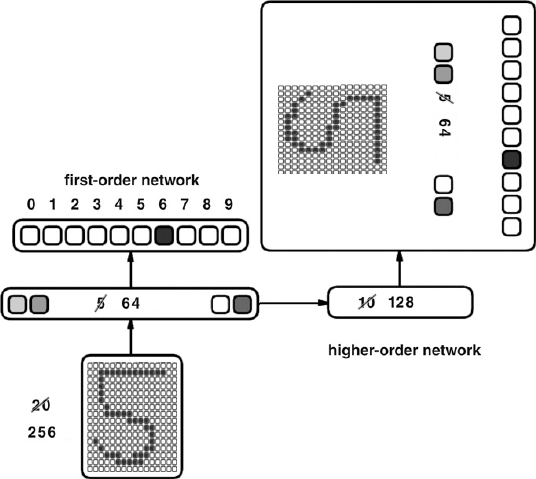
\includegraphics[width=220px]{data/expA3/schema.png}
      \end{center}
      
    \paragraph{Paramètres}
      \begin{center}
	\begin{tabular}{lr}
	  \begin{minipage}{230px}
	    \begin{itemize}
	      \item momentum : 0.5 sur les 2 réseaux
	      \item taux d'apprentissage : 0.1 sur les 2 réseaux
	      \item \textbf{1600 formes} de chiffres différents présentées (shuffle) \cite{Handwritten_256}
	      \item apprentissage 10 (formes) x 4000 (époques)
	    \end{itemize}
	  \end{minipage}
	  &
	  \begin{minipage}{230px}
	    \begin{itemize}
	      \item poids initialisés sur [-0.25 ; 0.25]
	      \item taux d'apprentissage constant
	      \item entrées valent 0 ou 1
	      \item sigmoïde à température 1
	      \item utilisation de biais
	    \end{itemize}
	  \end{minipage}
	\end{tabular}
      \end{center}

  
  \newpage
  \subsection{Résultats}
    \paragraph{Principaux}
      Analyse des performances
      \begin{center}
	\begin{tabular}{lr}
	  \hspace*{-1cm}
	  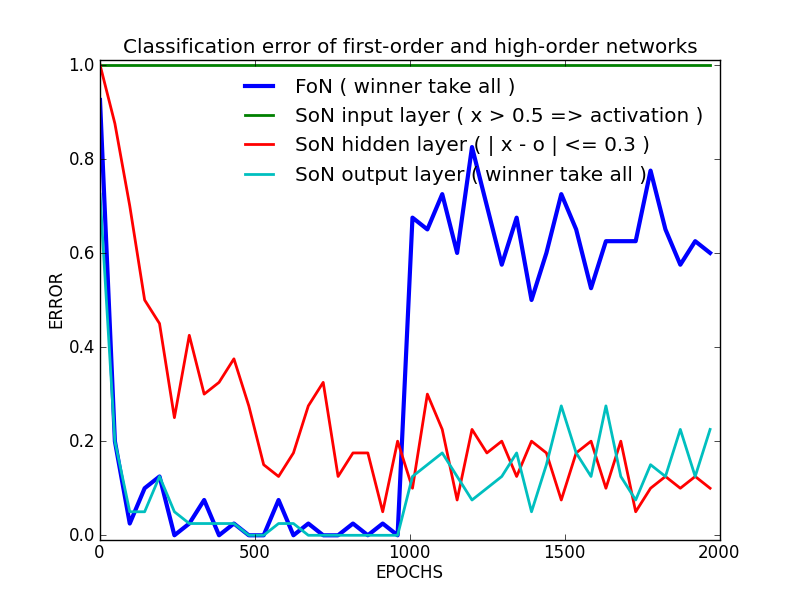
\includegraphics[width=250px]{data/expB5/err.png}
	  &
	  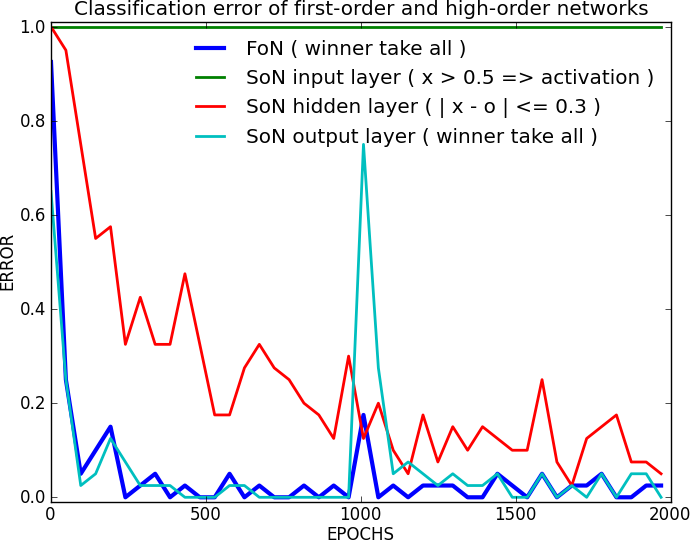
\includegraphics[width=250px]{data/expB5/err_block.png} \\
	  normal
	  &
	  poids figés
	\end{tabular}
      \end{center}
      \subparagraph{Notes}
	\begin{itemize}
	  \item l'erreur de classification représente le taux de mauvaises réponses pour les 10 formes présentées sur une époque
	  \item pour SoN input layer et hidden layer, un winner-take-all n'est pas possible (ce n'est pas de la classification, 
	  mais une duplication), il y a donc un seuil d'erreur qui ne doit pas être dépassé par un seul neurone
	\end{itemize}
      \subparagraph{Conclusion}
	\begin{itemize}
	  \item lorsque l'on fige les poids, le premier réseau arrive à se réadapter aux nouvelles tâches, mais s'ils ne sont
	  pas figés, il n'y arrive pas
	  \item la reproduction de la couche cachée par le second réseau ne pose pas de problème
	  \item lorsque l'on ne fige pas les poids, le second réseau est lui aussi instable
	  \item lorsque les poids sont figés, la couche de sortie a du mal à être totalement réapprise par le second réseau
	  
	\end{itemize}
    \paragraph{Secondaires}
       Analyse des performances RMS
      \begin{center}
	\begin{tabular}{lr}
	  \hspace*{-1cm}
	  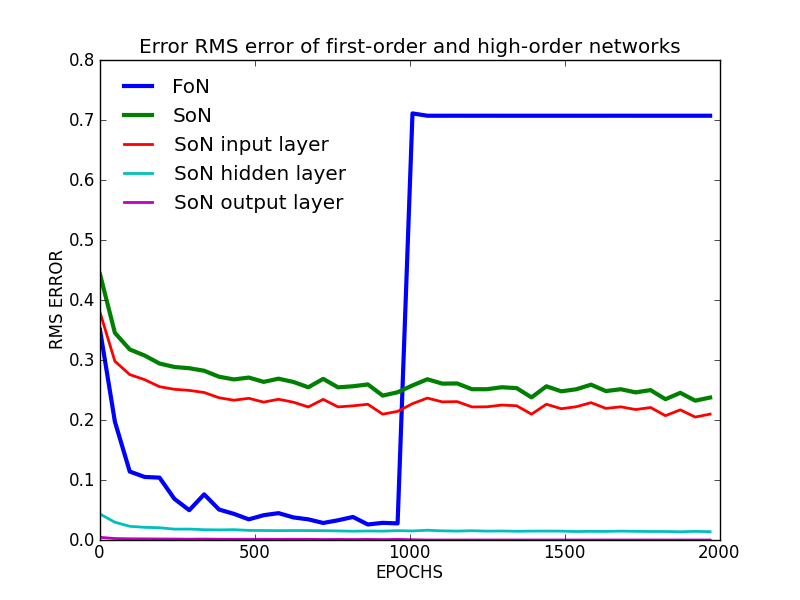
\includegraphics[width=250px]{data/expB5/rms.png}
	  &
	  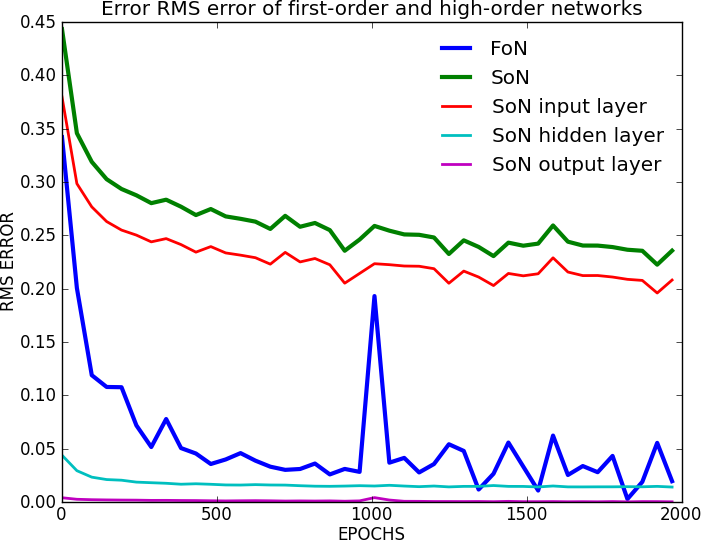
\includegraphics[width=250px]{data/expB5/rms_block.png} \\
	  normal
	  &
	  poids figés
	\end{tabular}
      \end{center} 
      \subparagraph{Notes}
	\begin{itemize}
	  \item formule utilisée pour RMS (cf. Formules~\nameref{rms})
	  \item les courbes SoN layer représentent les erreurs (du second réseaux) sur les couches à reproduire 
	  \item la courbe RMS verte (SoN) est la somme des 3 courbes SoN layer
	\end{itemize}
      \subparagraph{Conclusion}
	Ces courbes sont a peu près équivalentes à celles de classifications.

  \subsection{Conclusion}
    Le blocage des poids dans la couche cachée prouve la présence de représentations stables permettant le 
  transfert de tâche.
  
  Ces représentations contiennent ce qui caractérise la forme sans encore lui mettre un sens dessus.
  Il sait à quoi ressemble un 1 (dans la couche cachée) et lui met un donne le sens 1 (dans la couche de sortie).
  Il est donc facile de lui dire que finalement, cette représentation correspond à un 2, sans qu'il ait à réapprendre
  la forme entièrement.
  

  \newpage 
  \subsection{Formules}
    \paragraph{RMS} \label{rms}
  Pour une époque $e$ :
  \begin{center}
    \begin{large}
    $ rms_{e} = \sqrt{ \frac{1}{n} \sum \limits_{i=1}^{n} 
    ( o_{i,e} - d_{i} )^2 } $
    \end{large}
  $ with \left\lbrace \begin{array}{lll} n : number\ of\ neurons\ on\ the\ output\ 
  layer\\o_{i,e} : value\ obtained\ for\ the\ i^{th}\ neuron\ at\ the\ e^{th}\ epoch\\d_{i} : 
  value\ desired \ for\ the\ i^{th}\ neuron\end{array} \right.$
  \end{center}
    \paragraph{Descente de gradient} \cite{Touzet_1992} \\
  Construction de l'erreur : 
    \begin{center}
      $y_{i} = f'(a_i) \times ( d_i - x_i ) \ si\ i\ neurone\ de\ sortie $ \\
      $y_{i} = f'(a_i) \times \sum \limits_{k} ( w_{ki} \times y_k )\ si\ i\ neurone\ cache $
    \end{center}
  Mise à jour des poids :
    \begin{center}
      $w_{ij}(t+1) = w_{ij}(t) + learning\_rate \times y_{i} \times x_j + momentum \times 
      (w_{ij}(t) - w_{ij}(t-1) )$
    \end{center}
  Variables : 
    \begin{center}
      $\left\lbrace \begin{array}{lll} 
	f : fonction\ sigmoide \\
	x_i : valeur\ du\ neurone\ i\\
	d_i : valeur\ desire pour\ le\ neurone\ i\\
	a_i : somme\ pondere\ des\ poids\ du\ neurone\ i
      \end{array} \right.$
    \end{center}

\bibliographystyle{../pre-rapport/apalike}
\bibliography{../pre-rapport/biblio}
